\chapter{Extra Information}
This part of the report contains additional informations which might be useful in case the interested reader
would like to dive deeper into the topics and tools presented and possibly get hands-on himself.

\section{Digital Circuits Basics}
For an in-depth understanding of a computer to be complete, one would need to understand how each individual
component works, down to the transistor. Once a through understanding has been established, designing a new component
seems almost trivial, as there is almost always a right combination of primitive ~~tools'' available to do the job.
Here is a listing and description of those tools.


\subsection{Types of electrical circuits}
Electrical circuits can be broadly classified into two main categories: \emph{combinatorial} and \emph{sequential} circuits. \emph{Combinatorial circuits} are circuits without any internal state (no memory) which implement a certain logic function. A logic function maps binary inputs to binary outputs. They are implemented as cascading layers of \emph{logic gates.} The main techniques which can be used to transform a logic function into a combinatorial circuit are standard form reductions, map creations and adequate use of don't care conditions (input/output conditions which are considered to be invalid/ will never happen). \emph{Sequential circuits} are composed of two parts:
\begin{enumerate}
  \item A memory structure usually built out of \emph{flip flops}
  \item One ore more combinatorial circuits, implementing some logical functions
\end{enumerate}

\subsection{Logic Gates}
Logic gates are electronic devices usually built out of transistors which perform certain logic functions.
A \emph{logic function} is a function which maps binary inputs to binary outputs.

\subsection{The Transistor}
A transistor is an electronic device which allows the control of the flow of one current source through a second, potentially smaller current source. This serves as the basic component for creating more advanced electronic components like logic gates.
\begin{figure}[h]
  \centering
  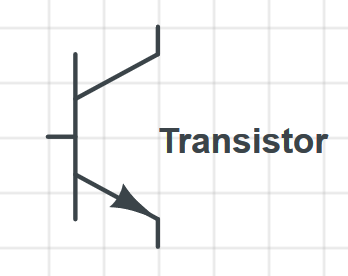
\includegraphics{trans}
  \caption{Transistor Symbol}
  \label{trans}
\end{figure}
Today, the most popular type of transistor and the most widley produced device in the world is the MOSFET \cite{chm2019mosfet}.


\subsection{Buffers}
Buffers are simple logic gates which just pass through the signal they receive.
\begin{table}[H]
\centering
\begin{tabular}{l|l}
\hline
\multicolumn{1}{|l|}{\textbf{A}} & \multicolumn{1}{l|}{\textbf{B}} \\ \hline
0                                & 0                               \\
1                                & 1
\end{tabular}
\caption{Truth table of a buffer}
\label{tab:buffer-table}
\end{table}
TO DO: ADD CIRCUIT DIAGRAM

\subsection{Inverters}
Inverters are similar in complexity to buffers. They invert the signal they receive.
\begin{table}[H]
\centering
\begin{tabular}{l|l}
\hline
\multicolumn{1}{|l|}{\textbf{A}} & \multicolumn{1}{l|}{\textbf{B}} \\ \hline
0                                & 1                               \\
1                                & 0
\end{tabular}
\caption{Truth table of an inverter}
\label{tab:inverter-table}
\end{table}
TO DO: ADD CIRCUIT DIAGRAM

\subsection{AND Gates}
And gates output a logic 1 only if all of their inputs are logic 1's.
\begin{table}[H]
\centering
\begin{tabular}{l|l|l}
\hline
\multicolumn{1}{|l|}{\textbf{A}} & \textbf{B} & \multicolumn{1}{l|}{\textbf{O}} \\ \hline
0                                & 0          & 0                               \\
1                                & 0          & 0                               \\
0                                & 1          & 0                               \\
1                                & 1          & 1
\end{tabular}
\caption{AND Gate Truth Table}
\label{tab:and-table}
\end{table}
TO DO: ADD CIRCUIT DIAGRAM

\subsection{OR Gates}
OR gates output a logic 1 if either of their inputs or both of them are logic 1's.
\begin{table}[H]
\centering
\begin{tabular}{l|l|l}
\hline
\multicolumn{1}{|l|}{\textbf{A}} & \textbf{B} & \multicolumn{1}{l|}{\textbf{O}} \\ \hline
0                                & 0          & 0                               \\
1                                & 0          & 1                               \\
0                                & 1          & 1                               \\
1                                & 1          & 1
\end{tabular}
\caption{OR Gate Truth Table}
\label{tab:or-table}
\end{table}
TO DO: ADD CIRCUIT DIAGRAM

\subsection{XOR Gates}
Exclusive OR, or XOR gates output a logic 1 only if either of their inputs is a 1, but not both.
\begin{table}[H]
\centering
\begin{tabular}{l|l|l}
\hline
\multicolumn{1}{|l|}{\textbf{A}} & \textbf{B} & \multicolumn{1}{l|}{\textbf{O}} \\ \hline
0                                & 0          & 0                               \\
1                                & 0          & 1                               \\
0                                & 1          & 1                               \\
1                                & 1          & 0
\end{tabular}
\caption{XOR Gate Truth Table}
\label{tab:xor-table}
\end{table}
TO DO: ADD CIRCUIT DIAGRAM

\subsection{NAND Gates}
A NAND gate is an inverted AND gate. This means it outputs a logic 1 in all situations except for when all of its inputs are logic 1's.
\begin{table}[H]
\centering
\begin{tabular}{l|l|l}
\hline
\multicolumn{1}{|l|}{\textbf{A}} & \textbf{B} & \multicolumn{1}{l|}{\textbf{O}} \\ \hline
0                                & 0          & 1                               \\
1                                & 0          & 1                               \\
0                                & 1          & 1                               \\
1                                & 1          & 0
\end{tabular}
\caption{NAND Gate Truth Table}
\label{tab:nand-table}
\end{table}
TO DO: ADD CIRCUIT DIAGRAM


\subsection{NOR Gates}
A NOR Gate is an inverted OR gate. This means it outputs a logic 1 only if all of its inputs are logic 0's.
NAND and NOR gates are considered \emph{universal gates}. This means that any logic circuit can be built exclusivley out of NAND or out of NOR gates.
\begin{table}[H]
\centering
\begin{tabular}{l|l|l}
\hline
\multicolumn{1}{|l|}{\textbf{A}} & \textbf{B} & \multicolumn{1}{l|}{\textbf{O}} \\ \hline
0                                & 0          & 1                               \\
1                                & 0          & 0                               \\
0                                & 1          & 0                               \\
1                                & 1          & 0
\end{tabular}
\caption{NOR Gate Truth Table}
\label{tab:nor-table}
\end{table}
TO DO: ADD CIRCUIT DIAGRAM

\subsection{Flip Flops}
Flip Flops are circuits usually built out of logic gates which can store one bit of information, i.e. they can be either on or off. There are many types of flip flops: RS-flip-flops (Reset-Set), D-flip-flops (Data), JK-flip flops (refined RS flip flops) and T flops (single input JK flip-flops). Each flip flop performs best in a certain scenario. Since they all implement de storage and retrieval of one bit of information, only the D-flip-flop (the most commonly used one) will be discussed. \\
TODO: ADD D FLIP FLOP DESC.
